\documentclass[12pt,a4paper]{report}

\usepackage[margin=1in]{geometry}
\usepackage{amsmath}
\usepackage{amssymb}
\usepackage{graphicx}
\usepackage{hyperref}
\usepackage{booktabs}
\usepackage{setspace}
\usepackage{algorithm}
\usepackage{algpseudocode}
\usepackage{tikz}
\usetikzlibrary{arrows.meta,positioning,shapes.geometric,calc}

\hypersetup{
    hidelinks
}

\newcommand{\chapterdesc}[1]{%
    \vspace{-0.6\baselineskip}
    \noindent\hspace*{1.5cm}\parbox{\dimexpr\textwidth-1.5cm\relax}{\textit{#1}}
    \par\vspace{0.3\baselineskip}
}

\begin{document}

\onehalfspacing

% ----------------------------
% Title page (styled like model PDF)
% ----------------------------
\begin{titlepage}
    \centering
    
\includegraphics[height=2.6cm]{bk.png}\par
    \vspace{0.6cm}
    {\large VIETNAM NATIONAL UNIVERSITY\par}
    {\large UNIVERSITY OF TECHNOLOGY\par}
    {\large FACULTY OF COMPUTER SCIENCE AND ENGINEERING\par}
    \vspace{1.5cm}
    {\large\bfseries - INTERNSHIP PROJECT 2 REPORT -\par}
    \vspace{1.0cm}
    {\Large\bfseries Enhancing FraudGNN-RL via Multi-modal Semantic Fusion for Adaptive Fraud Detection\par}
    \vspace{1.5cm}
    \begin{flushleft}
        \begin{tabular}{@{}l c l@{}}
            \textbf{Council}    & : & Computer Science \\
            \textbf{University} & : & Ho Chi Minh University of Technology \\
            \textbf{Faculty}    & : & Computer Science and Engineering \\
            \textbf{Instructor} & : & Prof. Quản Thành Thơ \\
            \textbf{Author}     & : & Đặng Thế Đông A (2570791)
        \end{tabular}
    \end{flushleft}
    \vfill
    {\large Ho Chi Minh City, May 2026\par}
\end{titlepage}

\clearpage
\pagenumbering{roman}

\chapter*{Declaration of Authenticity}
I declare that this internship report is my own work, conducted under the supervision of my instructor. The results and discussions presented in this report are original to this project context and have not been published previously in this form.

All materials, methods, and references adopted from prior works are properly cited in the References section. Any use of external ideas, datasets, and technical foundations is acknowledged in accordance with academic integrity requirements.

\clearpage
\chapter*{Acknowledgements}
I would like to express my sincere gratitude to my instructor and the members of the research group for their guidance, support, and valuable feedback throughout this internship.

I also thank my family and friends for their continuous encouragement during the implementation and writing process of this report.

\clearpage
\chapter*{Abstract}
This report presents an extension of the FraudGNN-RL framework for adaptive fraud detection under evolving transaction behavior. The core contribution is a transition from categorical entity embeddings to Multi-modal Semantic Modeling (M-SEM) using IEEE-CIS identity and device attributes as behavioral signals.

The proposed design directly targets identity camouflage and concept drift. The semantic branch is enhanced through cross-attention fusion between DeviceInfo and identity indicators, and the reinforcement learning component is used for adaptive weighting and threshold control. The framework combines temporal, spatial, and semantic channels in a unified graph model, with evaluation planned using AUC-ROC, AUC-PR, F1-score, and Recall@1\%.

\clearpage
\tableofcontents
\listoffigures
\listoftables
\clearpage

\pagenumbering{arabic}

\chapter{Introduction}
\chapterdesc{This chapter introduces the main fraud detection problem and explains why identity camouflage and concept drift are difficult in practice. It also presents the goals, scope, and overall structure of Internship Project 2.}

\section{Problem Statement}
Online payment fraud is the act of making or authorizing digital transactions through deception, such as using stolen credentials, synthetic identities, or compromised devices. Although the action often appears as a ``normal payment'' at checkout time, its accumulated impact is systemic: The Nilson Report estimates global payment card fraud losses at \$33.41 billion in 2024 \cite{global_fraud_loss_report}.

In practical terms, fraud rarely happens as a single dramatic event; it happens by blending in. A fraudster studies ordinary user behavior (purchase amount range, preferred merchant categories, usual device family, timing habits), then mimics these signals to avoid triggering simple alarms. This strategy is referred to in this report as \emph{identity camouflage}: the attacker does not only steal an account, but also imitates the account's expected digital footprint.

Another core property of fraud detection is \textbf{extreme class imbalance}. In real transaction streams, fraudulent samples are usually a tiny minority (often below 1\%), while legitimate payments dominate the dataset. This means a naive classifier can report very high accuracy simply by predicting ``legitimate'' for almost every case.

Formally, if $N_f$ is the number of fraud cases and $N_l$ is the number of legitimate cases, then typically:
\[
\frac{N_f}{N_f+N_l} \ll 0.01.
\]
Under this regime, plain accuracy
\[
\mathrm{Accuracy}=\frac{TP+TN}{TP+TN+FP+FN}
\]
can be misleading, because the large $TN$ term can mask poor fraud recall \cite{saito_pr_imbalanced}. Therefore, fraud modeling should emphasize imbalance-aware measures such as AUC-PR, F1-score, Recall, and Recall@1\% alert budget.

From a modeling perspective, this creates two linked challenges. First, static rules struggle because attackers can quickly adapt to fixed constraints and bypass deterministic thresholds \cite{rule_based_fraud}. Second, models that only inspect one view of data (only tabular attributes or only graph structure) miss subtle inconsistencies across time, relations, and device semantics. This internship therefore targets identity camouflage and concept drift as the primary barriers to reliable real-world fraud detection.

\section{Goals}
This internship focuses on extending FraudGNN-RL with multi-modal semantic fusion for adaptive and resilient detection. The project goals are:
\begin{itemize}
    \item Implement M-SEM to replace categorical semantic embeddings with multi-modal behavioral representations.
    \item Preserve and enhance RL-driven adaptive thresholding through DQN-based decision control.
    \item Improve temporal robustness to concept drift via chronological evaluation and cross-temporal testing.
    \item Validate gains using standard and operational fraud metrics.
\end{itemize}

\section{Scope}
This report concentrates on model and evaluation design for Internship Project 2. The implementation scope includes IEEE-CIS data preprocessing, semantic encoder integration, dynamic RL-driven modality weighting, and comparison with selected baselines.

The current scope excludes production deployment, online serving optimization, and institution-scale federated system rollout.

\section{Internship Project 2 Structure}
The remainder of this report is organized as follows:
\begin{itemize}
    \item Chapter 2 provides the theoretical background for GNNs, DQN, and attention mechanisms.
    \item Chapter 3 presents related works under a technique taxonomy.
    \item Chapter 4 introduces the initial proposal solutions of this internship.
    \item Chapter 5 summarizes the conclusion and implementation schedule.
\end{itemize}

\chapter{Theoretical Background}
\chapterdesc{This chapter presents the theoretical foundation used in this internship, including graph modeling, temporal dynamics, spatial message passing, semantic fusion, reinforcement learning, and federated learning. These concepts form the technical basis for the proposed framework in later chapters.}

\section{Graph Foundations and Heterogeneous Modeling}
\subsection{General Definition of a Graph}
A graph is a mathematical structure used to represent objects and relationships:
\begin{equation}
\mathcal{G}=(\mathcal{V},\mathcal{E}),
\end{equation}
where $\mathcal{V}$ is the set of nodes (objects) and $\mathcal{E}$ is the set of edges (relations between nodes). In fraud detection, this abstraction is useful because a transaction is rarely independent; its risk depends on how it connects to identities, devices, merchants, and historical events.

\subsection{Homogeneous vs. Heterogeneous Graphs}
In a \textbf{homogeneous graph}, all nodes share one type and all edges share one relation type. This is convenient for simple social or citation networks, but it forces semantically different entities to be treated as if they were identical.

In a \textbf{heterogeneous graph}, both nodes and edges can have multiple types. Formally, let $\phi(v)$ map node $v$ to a node type and $\psi(e)$ map edge $e$ to a relation type. If the number of node types or edge types is greater than one, the graph is heterogeneous:
\[
|\mathcal{A}|>1 \quad \text{or} \quad |\mathcal{R}|>1,
\]
where $\mathcal{A}$ is the node-type set and $\mathcal{R}$ is the relation-type set.

\subsection{Why Heterogeneous Graphs Are Necessary for IEEE-CIS}
The IEEE-CIS fraud dataset is intrinsically multi-entity and multi-relation: users, transactions, merchants, and devices have different semantics and should not be collapsed into a single node type. Their links also mean different things (e.g., ownership, payment routing, device source). If these are flattened into a homogeneous graph, type-specific meaning is lost and message passing can mix incompatible signals.

Therefore, heterogeneous modeling is not only a design preference but a structural requirement for preserving fraud-relevant semantics, especially when detecting identity camouflage across entity boundaries.

\subsection{IEEE-CIS Instantiation in This Report}
After defining the graph type, we instantiate IEEE-CIS as:
\begin{equation}
\mathcal{V}=V_u \cup V_t \cup V_m \cup V_d,
\label{eq:hgraph-nodes}
\end{equation}
where $V_u, V_t, V_m, V_d$ denote user, transaction, merchant, and device nodes, respectively.

Edge sets encode typed relations:
\begin{equation}
\mathcal{E}=\mathcal{E}_{u,t}\cup\mathcal{E}_{t,m}\cup\mathcal{E}_{d,t},
\label{eq:hgraph-edges}
\end{equation}
where $\mathcal{E}_{u,t}$ represents ownership/initiator links, $\mathcal{E}_{t,m}$ represents transaction-merchant links, and $\mathcal{E}_{d,t}$ represents device-source links. This structure enables cross-entity dependency learning that is difficult to capture with tabular features alone.

In IEEE-CIS preprocessing, each node type is instantiated using proxy keys that approximate real entities. The most important identity proxy for user-level continuity is the composite key
\[
\texttt{UserProxy} = (\texttt{card1},\ldots,\texttt{card6},\texttt{addr1}),
\]
which captures payment instrument and coarse location consistency. A transaction node $V_t$ is represented by each \texttt{TransactionID}. Merchant nodes $V_m$ are built from merchant-facing attributes (e.g., \texttt{ProductCD} and acceptance context), while device nodes $V_d$ are constructed from \texttt{DeviceInfo}/\texttt{DeviceType}. These proxy mappings are crucial because they convert noisy raw fields into explicit actor relationships that support relational reasoning under camouflage attempts.

\begin{figure}[htbp]
\centering
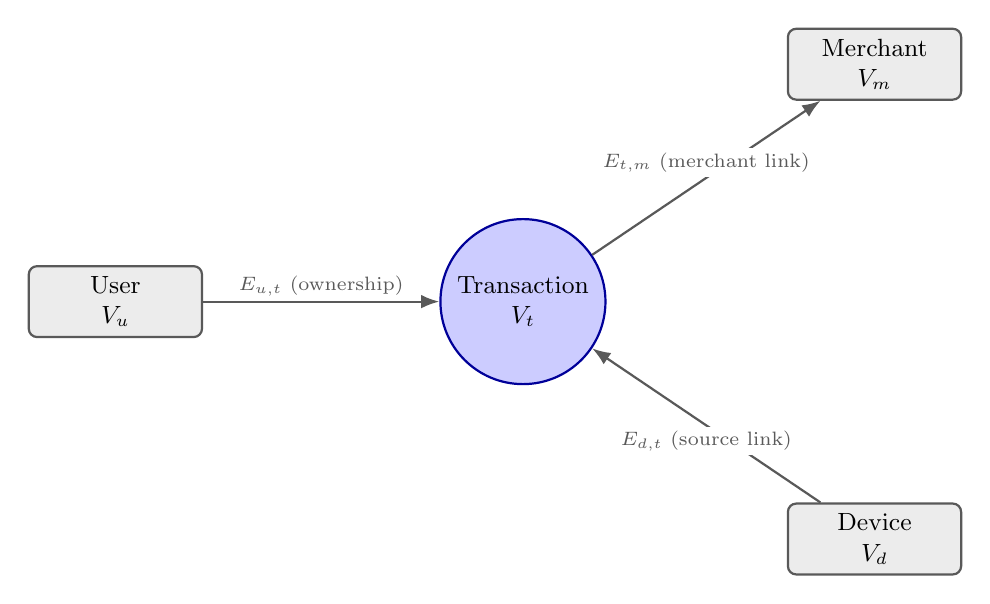
\begin{tikzpicture}[
  >=Latex,
  node distance=2.2cm,
  every node/.style={font=\small},
  trans/.style={circle, draw=blue!60!black, fill=blue!20, thick, minimum size=1.4cm, align=center},
  ent/.style={rectangle, rounded corners=3pt, draw=gray!70!black, fill=gray!15, thick, minimum width=2.2cm, minimum height=0.9cm, align=center},
  edgeLabel/.style={midway, fill=white, inner sep=1.5pt, font=\scriptsize}
]
  \node[trans] (vt) {Transaction\\$V_t$};
  \node[ent, left=3cm of vt] (vu) {User\\$V_u$};
  \node[ent, above right=1.8cm and 2.6cm of vt] (vm) {Merchant\\$V_m$};
  \node[ent, below right=1.8cm and 2.6cm of vt] (vd) {Device\\$V_d$};

  \draw[->, thick, gray!70!black] (vu) -- node[edgeLabel, above] {$E_{u,t}$ (ownership)} (vt);
  \draw[->, thick, gray!70!black] (vt) -- node[edgeLabel, above] {$E_{t,m}$ (merchant link)} (vm);
  \draw[->, thick, gray!70!black] (vd) -- node[edgeLabel, below] {$E_{d,t}$ (source link)} (vt);
\end{tikzpicture}
\caption{H-Graph schema with typed actors (user, transaction, merchant, device) and relation edges.}
\label{fig:heterogeneous-graph-schema}
\end{figure}

\section{Introduction to Graph Neural Networks (GNNs)}
Graph Neural Networks (GNNs) are a family of models designed to learn representations directly from graph-structured data. Instead of treating each sample as independent, GNNs assume that a node's meaning depends on both its own attributes and the context provided by connected neighbors.

\subsection{Neighborhood Aggregation}
At a high level, each node updates its representation by collecting information from its local neighborhood. This process is usually called \emph{neighborhood aggregation}: node $i$ gathers messages from neighbors $j \in \mathcal{N}(i)$, summarizes them, and combines the summary with its current state.

The key intuition is local consistency: if nearby nodes or relations look suspicious together, the target node should inherit part of that signal. In fraud detection, this allows one transaction to be interpreted in the context of related devices, linked identities, and merchant interaction patterns.

\subsection{General Message Passing Framework}
Most GNN layers can be written in two generic steps at layer $l$:
\begin{equation}
\mathbf{m}_i^{(l)}=
\mathrm{AGG}^{(l)}\left(
\left\{
\phi^{(l)}\!\left(
\mathbf{h}_i^{(l)},\mathbf{h}_j^{(l)},\mathbf{e}_{ij}
\right)
\; \middle|\; j\in\mathcal{N}(i)
\right\}
\right),
\label{eq:general-message-passing-agg}
\end{equation}
\begin{equation}
\mathbf{h}_i^{(l+1)}=
\psi^{(l)}\!\left(\mathbf{h}_i^{(l)},\mathbf{m}_i^{(l)}\right),
\label{eq:general-message-passing-update}
\end{equation}
where $\mathbf{h}_i^{(l)}$ is the node embedding, $\mathbf{e}_{ij}$ is optional edge information, $\phi^{(l)}$ defines message construction, $\mathrm{AGG}^{(l)}$ is a permutation-invariant aggregator (such as sum, mean, max, or attention-weighted sum), and $\psi^{(l)}$ is the update function.

Stacking multiple layers expands the receptive field: after $L$ layers, node $i$ can incorporate information up to approximately $L$ hops away. This general paradigm is the foundation for the specific GNN layers used later in this chapter, such as attention-based aggregation and temporal-spatial fusion.

\section{Temporal Dynamics (GRU and Time-decaying Attention)}
Fraud events arrive as sequences, not isolated points. A model must therefore remember earlier context (e.g., gradual probing behavior) while still reacting to recent changes. The Gated Recurrent Unit (GRU) is a recurrent architecture designed for this purpose.

Compared with standard RNNs, GRUs are stronger in long-range temporal modeling because they use gates to regulate memory flow. This gating mechanism helps mitigate the vanishing gradient problem of vanilla RNNs, allowing useful historical information to persist across longer transaction sequences.

For each timestep $k$ with input $\mathbf{x}_k$ and previous hidden state $\mathbf{h}_{k-1}$, the GRU computes:
\begin{equation}
\mathbf{z}_k = \sigma\!\left(W_z\mathbf{x}_k + U_z\mathbf{h}_{k-1} + \mathbf{b}_z\right), \quad
\mathbf{r}_k = \sigma\!\left(W_r\mathbf{x}_k + U_r\mathbf{h}_{k-1} + \mathbf{b}_r\right),
\end{equation}
\begin{equation}
\tilde{\mathbf{h}}_k = \tanh\!\left(W_h\mathbf{x}_k + U_h(\mathbf{r}_k \odot \mathbf{h}_{k-1}) + \mathbf{b}_h\right),
\end{equation}
\begin{equation}
\mathbf{h}_k = (1-\mathbf{z}_k)\odot \mathbf{h}_{k-1} + \mathbf{z}_k \odot \tilde{\mathbf{h}}_k.
\end{equation}
Here, $\mathbf{z}_k$ is the update gate (how much new information to write), and $\mathbf{r}_k$ is the reset gate (how much past information to forget when forming a candidate state).

At the model level, this temporal encoding is summarized as:
\begin{equation}
\mathbf{h}_k = \mathrm{GRU}(\mathbf{x}_k,\mathbf{h}_{k-1}),
\label{eq:gru-temporal}
\end{equation}
where $\mathbf{x}_k$ is the feature representation of the $k$-th event in chronological order.

Fraud behavior is not stationary. New social-engineering scripts, bot frameworks, and laundering paths continuously appear, while old tactics fade. This evolving pattern is known as \emph{concept drift}: the statistical relationship between observed signals and fraud labels changes over time. As a result, older observations become progressively less informative for present-day decisions.

Because recent behavior should dominate current risk estimation, a time-decay weighting mechanism is introduced:
\begin{equation}
\alpha_k =
\frac{\exp\left(-\beta (t_{\mathrm{now}}-t_k)\right)}
{\sum_{l \in \mathcal{H}_i}\exp\left(-\beta (t_{\mathrm{now}}-t_l)\right)},
\label{eq:time-decay}
\end{equation}
where $\beta>0$ is the decay factor and $\mathcal{H}_i$ is the historical set for node $i$. Equation~\eqref{eq:time-decay} operationalizes concept drift by down-weighting stale evidence. A larger $\beta$ makes decay more aggressive (strong recency bias), while a smaller $\beta$ keeps longer historical memory.

\section{Spatial Contextualization (GAT and Message Passing)}
Spatial learning is performed through message passing over multi-hop neighborhoods. For node $i$, neighborhood aggregation is:
\begin{equation}
\mathbf{m}_i^{(l)} = \sum_{j \in \mathcal{N}(i)} \alpha_{ij}^{(l)} W^{(l)} \mathbf{h}_j^{(l)},
\end{equation}
followed by
\begin{equation}
\mathbf{h}_i^{(l+1)} = \sigma\left(W_0^{(l)}\mathbf{h}_i^{(l)} + \mathbf{m}_i^{(l)}\right).
\end{equation}

Here, $\alpha_{ij}^{(l)}$ are Graph Attention Network (GAT) coefficients that prioritize important neighbors:
\begin{equation}
\alpha_{ij}^{(l)} =
\mathrm{softmax}_j\left(
\mathrm{LeakyReLU}\left(
\mathbf{a}^{\top}
\left[W^{(l)}\mathbf{h}_i^{(l)} \,\|\, W^{(l)}\mathbf{h}_j^{(l)}\right]
\right)
\right).
\end{equation}
This mechanism allows suspicious relations to receive higher influence than routine interactions.

\section{Multi-modal Representation Learning (Cross-Attention for M-SEM)}
The M-SEM layer can be interpreted as a \emph{cross-attention fusion mechanism}. In manual analysis, investigators assess whether transaction behavior is consistent with the claimed device context. M-SEM formalizes this process computationally: device context is used as the query stream, while behavioral indicators provide key/value information for compatibility estimation.

This design is important for anti-camouflage robustness. Simple labels (e.g., one-hot device categories) are easy to spoof and often too coarse, while hardware/software strings in \texttt{DeviceInfo} carry richer device-fingerprint traces (browser-engine variants, OS-build signatures, driver stack artifacts, formatting idiosyncrasies). These latent signatures are harder to imitate consistently across time.

Formally, the semantic branch shifts from categorical lookup embeddings to cross-modal behavioral representation. Device context and identity indicators are fused through cross-attention. Let $E_{\mathrm{dev}}$ and $E_{\mathrm{id}}$ denote the device and identity-indicator streams:
\begin{equation}
E_{\mathrm{dev}} = f_{\mathrm{text}}(\texttt{DeviceInfo}), \qquad
E_{\mathrm{id}} = f_{\mathrm{MLP}}(\texttt{id\_12},\ldots,\texttt{id\_38}),
\end{equation}
where $f_{\mathrm{text}}$ is a text encoder for unstructured device strings and $f_{\mathrm{MLP}}$ is a multi-layer perceptron for numerical/categorical identity indicators.
\begin{equation}
Q = W_Q E_{\mathrm{dev}}, \quad K = W_K E_{\mathrm{id}}, \quad V = W_V E_{\mathrm{id}}.
\end{equation}
Then:
\begin{equation}
M_{\mathrm{SEM}}(i)=\mathrm{Softmax}\left(\frac{QK^\top}{\sqrt{d_k}}\right)V.
\end{equation}
In this formulation, $Q$ from device context determines which behavioral dimensions in $K,V$ are most compatible with the claimed hardware fingerprint. The resulting embedding captures cross-modal consistency, making identity camouflage more detectable than with static category encodings.

\begin{figure}[htbp]
\centering
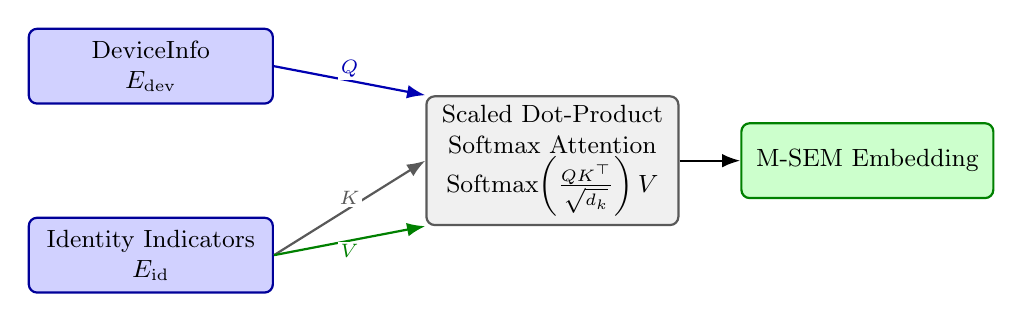
\begin{tikzpicture}[
  >=Latex,
  every node/.style={font=\small},
  src/.style={rectangle, rounded corners=3pt, draw=blue!60!black, fill=blue!18, thick, minimum width=3.1cm, minimum height=0.95cm, align=center},
  proc/.style={rectangle, rounded corners=3pt, draw=gray!70!black, fill=gray!12, thick, minimum width=3.2cm, minimum height=1.2cm, align=center},
  outbox/.style={rectangle, rounded corners=3pt, draw=green!50!black, fill=green!20, thick, minimum width=3.2cm, minimum height=0.95cm, align=center},
  tag/.style={font=\scriptsize, fill=white, inner sep=1pt}
]
  \node[src] (edev) at (0,1.2) {DeviceInfo\\$E_{\mathrm{dev}}$};
  \node[src] (eid) at (0,-1.2) {Identity Indicators\\$E_{\mathrm{id}}$};

  \node[proc] (attn) at (5.1,0) {Scaled Dot-Product\\Softmax Attention\\$\mathrm{Softmax}\!\left(\frac{QK^\top}{\sqrt{d_k}}\right)V$};
  \node[outbox] (msem) at (9.1,0) {M-SEM Embedding};

  \draw[->, thick, blue!70!black] (edev.east) -- node[tag, above] {$Q$} (attn.north west);
  \draw[->, thick, gray!70!black] (eid.east) -- node[tag, above] {$K$} (attn.west);
  \draw[->, thick, green!50!black] (eid.east) -- node[tag, below] {$V$} (attn.south west);

  \draw[->, thick] (attn.east) -- (msem.west);
\end{tikzpicture}
\caption{M-SEM cross-attention: device context ($Q$) attends to behavioral indicators ($K,V$).}
\label{fig:msem-cross-attention}
\end{figure}

\section{Adaptive Reinforcement Learning (DQN for Thresholding)}
\subsection{Agent-Environment Loop}
Reinforcement Learning (RL) is based on a repeated interaction loop between an \emph{agent} and an \emph{environment}. At each time step $t$, the agent observes a state $s_t$, selects an action $a_t$, then receives a reward $r_t$ and the next state $s_{t+1}$.

In this internship, the agent is the DQN controller and the environment is the fraud classification system. The action corresponds to adaptive threshold/channel control, while the reward reflects detection quality and false-positive cost.

\subsection{MDP Foundations}
The formal foundation of this loop is a Markov Decision Process (MDP):
\[
\mathcal{M}=(\mathcal{S},\mathcal{A},P,R,\gamma),
\]
where $\mathcal{S}$ is the state space, $\mathcal{A}$ is the action space, $P(s'|s,a)$ is the transition probability, $R(s,a)$ is the reward function, and $\gamma\in[0,1)$ is the discount factor.

Core elements are:
\begin{itemize}
    \item \textbf{State} ($s_t$): current risk context (node embedding, recent outcomes, and channel reliability).
    \item \textbf{Action} ($a_t$): control decision (e.g., threshold adjustment and channel reweighting).
    \item \textbf{Reward} ($r_t$): immediate feedback that encourages high fraud recall and penalizes costly false positives.
\end{itemize}
The objective is to learn a policy $\pi(a|s)$ that maximizes expected discounted return:
\[
G_t=\sum_{k=0}^{\infty}\gamma^k r_{t+k+1}.
\]

\subsection{DQN for Adaptive Thresholding}
FraudGNN-RL instantiates this MDP with Deep Q-Learning, where the agent learns an action-value function $Q(s,a)$ to estimate the long-term utility of each control action under a given fraud-risk state.

Operationally, each action $a_t$ corresponds to a threshold/channel-control decision. Rather than using one fixed threshold for all periods, the policy adapts decisions according to current context (transaction graph embedding, recent prediction behavior, and drift intensity). This makes the decision layer responsive to non-stationary fraud patterns.

At inference time, the controller selects:
\[
a_t^*=\arg\max_{a} Q_{\theta}(s_t,a),
\]
which means it chooses the action with the highest estimated future return. In this report, that return is shaped by the reward design in the next subsection and optimized through the DQN objective in Equation~\eqref{eq:dqn-loss}.

\subsection{Reward Function Design}
The reward function $r_t$ is designed to align RL decisions with operational fraud objectives: catch more fraudulent transactions while avoiding unnecessary alarms for legitimate users.

At each decision step, outcomes can be mapped to confusion-matrix events and weighted as:
\begin{equation}
r_t =
\lambda_{\mathrm{TP}}\cdot \mathbb{1}[\mathrm{TP}]
\;+\;
\lambda_{\mathrm{TN}}\cdot \mathbb{1}[\mathrm{TN}]
\;-\;
\lambda_{\mathrm{FP}}\cdot \mathbb{1}[\mathrm{FP}]
\;-\;
\lambda_{\mathrm{FN}}\cdot \mathbb{1}[\mathrm{FN}],
\end{equation}
where $\lambda_{\mathrm{TP}},\lambda_{\mathrm{TN}},\lambda_{\mathrm{FP}},\lambda_{\mathrm{FN}}>0$ are task-dependent coefficients.

In practice, the policy receives a positive reward when it correctly flags fraud (True Positive), a smaller or neutral reward for correct legitimate decisions (True Negative), and explicit penalties for false alarms (False Positive) and missed fraud (False Negative). Because false positives create operational friction and customer dissatisfaction, the $\lambda_{\mathrm{FP}}$ term is configured as a direct penalty in the reward.

\subsection{DQN Loss and Experience Replay Buffer}
The Q-function estimates long-term value for each state-action pair, and is optimized with replay memory and a target network:
\begin{equation}
\mathcal{L}_{\mathrm{DQN}}(\theta)=
\mathbb{E}_{(s,a,r,s')\sim\mathcal{D}}
\left[
\left(r+\gamma \max_{a'}Q_{\theta^-}(s',a')-Q_{\theta}(s,a)\right)^2
\right].
\label{eq:dqn-loss}
\end{equation}
Equation~\eqref{eq:dqn-loss} minimizes the temporal-difference error between current Q-estimates and bootstrap targets.

The experience replay buffer $\mathcal{D}$ stores transitions $(s_t,a_t,r_t,s_{t+1})$ and samples mini-batches uniformly (or by priority) during training. This breaks harmful short-term correlation in online trajectories, improves sample efficiency by reusing past experiences, and stabilizes DQN optimization.

This adaptive control is essential when static thresholds fail under rapidly changing fraud patterns, particularly during abrupt drift events and emerging zero-day tactics.

\begin{figure}[htbp]
\centering
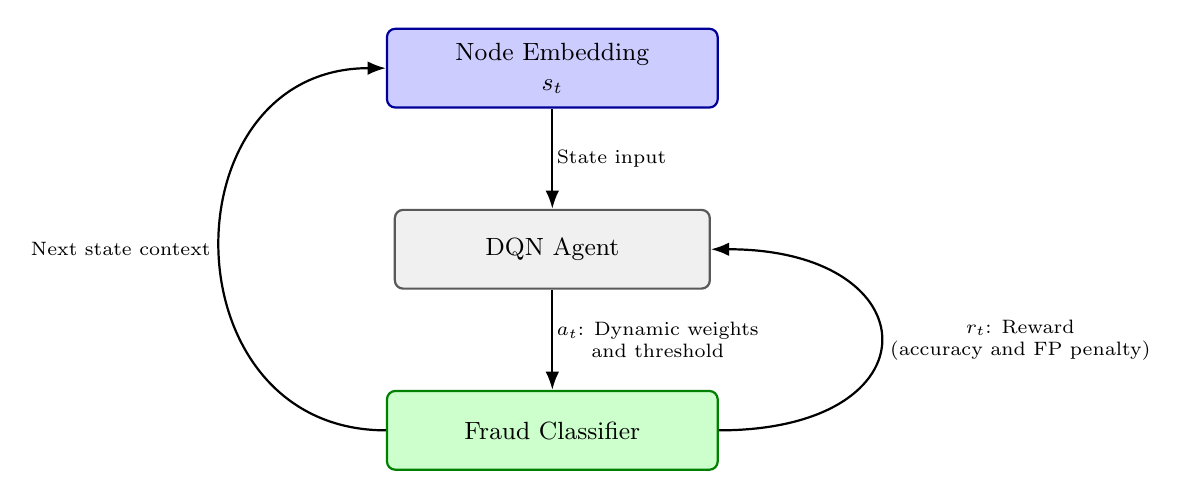
\begin{tikzpicture}[
  >=Latex,
  every node/.style={font=\small},
  block/.style={rectangle, rounded corners=3pt, draw=gray!70!black, fill=gray!12, thick, minimum width=4.0cm, minimum height=1.0cm, align=center},
  state/.style={rectangle, rounded corners=3pt, draw=blue!60!black, fill=blue!20, thick, minimum width=4.2cm, minimum height=1.0cm, align=center},
  env/.style={rectangle, rounded corners=3pt, draw=green!50!black, fill=green!20, thick, minimum width=4.2cm, minimum height=1.0cm, align=center},
  lab/.style={font=\scriptsize, fill=white, inner sep=1.2pt, align=center}
]
  \node[state] (state) at (0,5.8) {Node Embedding\\$s_t$};
  \node[block] (dqn) at (0,3.5) {DQN Agent};
  \node[env] (cls) at (0,1.2) {Fraud Classifier};

  \draw[->, thick] (state.south) -- node[lab, right] {State input} (dqn.north);
  \draw[->, thick] (dqn.south) -- node[lab, right] {$a_t$: Dynamic weights\\and threshold} (cls.north);

  \draw[->, thick]
    (cls.east) .. controls +(2.8,0) and +(2.8,0) ..
    node[lab, right, xshift=2pt] {$r_t$: Reward\\(accuracy and FP penalty)} (dqn.east);

  \draw[->, thick]
    (cls.west) .. controls +(-2.8,0) and +(-2.8,0) ..
    node[lab, left, xshift=-2pt] {Next state context} (state.west);
\end{tikzpicture}
\caption{DQN loop for state-aware threshold and channel-weight adaptation.}
\label{fig:dqn-adaptive-loop}
\end{figure}

\section{Privacy-Preserving Federated Learning (FedAvg)}
Even when experiments are centralized, the theoretical foundation follows the original FraudGNN-RL setting with Federated Averaging (FedAvg). Multiple institutions train local models without sharing raw transactions. A central coordinator aggregates local parameters:
\begin{equation}
\mathbf{w}^{(r+1)}=
\sum_{k=1}^{K}\frac{n_k}{\sum_{j=1}^{K}n_j}\mathbf{w}_k^{(r+1)},
\end{equation}
where $\mathbf{w}_k^{(r+1)}$ is client $k$'s updated model at round $r+1$, and $n_k$ is its local sample size. This preserves data privacy while improving global fraud intelligence across domains.

\chapter{Related Works (Historical Evolution)}
\chapterdesc{This chapter reviews the historical evolution of fraud detection methods, from rule-based systems to deep sequential models, graph neural networks, and RL-augmented frameworks. It highlights the research gap that motivates the proposed multi-modal semantic extension.}

\section{Fraud Taxonomy: Threat Types That Motivate Model Design}
\label{sec:fraud-taxonomy}
Two fraud classes are central to this report. \textbf{Account Takeover (ATO)} refers to the hijacking of a specific legitimate identity (real cardholder/account), typically via credential theft, SIM swap, malware, or social engineering. ATO signals may evolve gradually, because attackers probe limits before escalating transaction value.

\textbf{Zero-Day Fraud} refers to newly emerging attack tactics that are not represented in the model's recent training distribution. In deployment, this appears as sudden behavior shifts (new device emulation stack, new merchant route abuse, or novel laundering cadence) that invalidate static assumptions. These definitions provide the threat lens for evaluating temporal robustness and adaptation quality.

\section{Rule-Based and Statistical Foundations (Simple but Brittle)}
Early fraud detection systems relied on expert-crafted rules and manually designed business constraints, for example flagging transactions that occur in geographically distant locations within a short time window \cite{rule_based_fraud}. These systems are highly interpretable and easy to audit, but they are static and brittle: adaptation to new fraud patterns requires continuous manual updates by domain experts.

Classical statistical models, including logistic regression and early data-mining pipelines, introduced partial automation and probabilistic scoring \cite{logistic_fraud,datamining_fraud}. However, these approaches often underfit highly non-linear interactions and suffer under severe class imbalance conditions (such as low fraud prevalence in large-scale datasets like IEEE-CIS \cite{ieee_cis_dataset}), limiting robustness in real-world deployment.

\section{Sequential Deep Models (Temporal but Isolated)}
Deep sequential models, especially RNN/LSTM families, were introduced to capture temporal dependencies in user spending behavior \cite{rnn_fraud,lstm_fraud}. Hybrid designs such as AdaBoost-LSTM combined ensemble learning with sequence encoders to improve sensitivity to evolving fraudulent trajectories \cite{adaboost_lstm}.

Time-aware variants (e.g., T-LSTM and HAInt-LSTM) further modified recurrent gating with elapsed-time signals so that outdated patterns decay and recent behaviors dominate model memory \cite{t_lstm,haint_lstm}. Although these architectures improve temporal fidelity, they mostly process transactions as isolated sequences and do not explicitly encode cross-entity relational structure among users, merchants, and devices.

\section{Graph Neural Networks (Relational View of Fraud Ecosystems)}
Graph Neural Networks addressed the relational gap by representing fraud ecosystems as interconnected heterogeneous graphs \cite{gnn_fraud_hetero}. Spatial-temporal models such as STGN introduced time-aware and location-aware gating to jointly model neighborhood interactions and chronological behavior shifts \cite{stgn}.

TbHGN extended this direction through hierarchical extraction, separating feature-oriented and transaction-oriented encoders before interaction, which improved representation granularity \cite{tbhgn}. More recent approaches such as TH-GCL incorporated contrastive learning to align temporal and structural graph views, improving robustness under sparse labels and enhancing sensitivity to zero-day anomalies \cite{th_gcl}.

\section{Adaptive RL-Augmented Frameworks (Context-Aware Decision Policies)}
The latest trend combines graph representation learning with reinforcement learning to handle concept drift explicitly \cite{dqn}. FraudGNN-RL uses a Deep Q-Network agent to observe node-level embeddings and adaptively adjust decision thresholds, consistently outperforming static-threshold baselines across dynamic datasets \cite{fraudgnn_rl}.

Federated and multi-agent extensions, such as FraudSentinel, allocate specialized agents to account, device, and payment channels, enabling cross-marketplace learning while avoiding raw-data sharing \cite{fraudsentinel,fedavg}. However, a gap remains across much of this evolution: semantics are often represented with shallow categorical labels. Such shallow semantics are vulnerable to identity camouflage, motivating the multi-modal behavioral-device fusion strategy proposed in this report.

\chapter{Initial Proposal Solutions}
\chapterdesc{This chapter presents the initial solutions of this internship, including the M-SEM semantic layer, dynamic RL-driven channel weighting, cross-temporal robustness evaluation, and the epoch-based training strategy. It explains how each solution contributes to adaptive fraud detection under evolving attack behavior.}

\section{Solution 1: M-SEM Layer}
Solution 1 directly targets the identity camouflage mechanism introduced in Chapter 1. Under camouflage, adversaries attempt to imitate visible account attributes while failing to reproduce deeper cross-modal consistency between hardware traces and behavioral signatures.

To operationalize this defense, we propose a Multi-modal Semantic Modeling (M-SEM) layer that fuses DeviceInfo strings and identity indicators. Let $E_{\mathrm{dev}}$ be the device embedding and $E_{\mathrm{id}}$ be the identity-indicator embedding. Cross-attention fusion is:
\begin{equation}
M_{\mathrm{SEM}}(i)=\mathrm{Softmax}\left(\frac{QK^\top}{\sqrt{d_k}}\right)V,
\end{equation}
where $Q=W_QE_{\mathrm{dev}}$, $K=W_KE_{\mathrm{id}}$, and $V=W_VE_{\mathrm{id}}$.

Operationally, this acts as a cross-attention fusion mechanism: device-context queries (through $Q$) attend to behavioral indicators ($K,V$) to evaluate whether the current connection pattern is typical for that hardware profile. This design is expected to expose camouflage attempts where high-level labels appear legitimate but latent device-behavior coupling is inconsistent.

The TSSGC update is then:
\begin{equation}
h_i^{(l+1)}=\sigma\left(
W_t^{(l)}\cdot TEMP(i)+
W_s^{(l)}\cdot SPAT(i)+
W_m^{(l)}\cdot M_{\mathrm{SEM}}(i)+
b^{(l)}
\right).
\end{equation}

\section{Solution 2: Dynamic RL-driven Weighting}
The DQN agent observes the current node embedding and transaction context, then outputs dynamic fusion weights for Spatial, Temporal, and Semantic channels. This allows adaptive channel emphasis under changing fraud behavior and supports robust threshold control.

\begin{figure}[htbp]
\centering
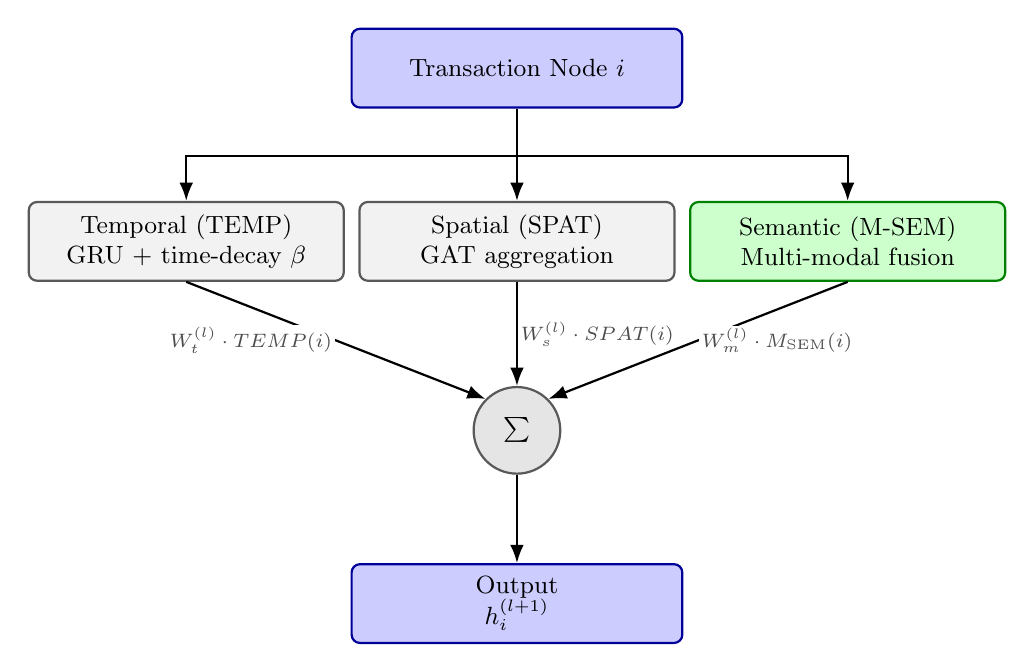
\begin{tikzpicture}[
  >=Latex,
  every node/.style={font=\small},
  block/.style={rectangle, rounded corners=3pt, draw=gray!70!black, fill=gray!10, thick, minimum width=4.0cm, minimum height=1.0cm, align=center},
  io/.style={rectangle, rounded corners=3pt, draw=blue!60!black, fill=blue!20, thick, minimum width=4.2cm, minimum height=1.0cm, align=center},
  sem/.style={rectangle, rounded corners=3pt, draw=green!50!black, fill=green!20, thick, minimum width=4.0cm, minimum height=1.0cm, align=center},
  merge/.style={circle, draw=gray!70!black, fill=gray!20, thick, minimum size=1.1cm},
  lab/.style={font=\scriptsize, text=gray!60!black, fill=white, inner sep=1pt, align=center}
]
  \node[io] (in) at (0,5.8) {Transaction Node $i$};
  \node[block] (temp) at (-4.2,3.6) {Temporal (TEMP)\\GRU + time-decay $\beta$};
  \node[block] (spat) at (0,3.6) {Spatial (SPAT)\\GAT aggregation};
  \node[sem]   (msem) at (4.2,3.6) {Semantic (M-SEM)\\Multi-modal fusion};
  \node[merge] (sum) at (0,1.2) {$\sum$};
  \node[io] (out) at (0,-1.0) {Output\\$h_i^{(l+1)}$};

  \draw[->, thick] (in.south) -- ++(0,-0.6) -| (temp.north);
  \draw[->, thick] (in.south) -- (spat.north);
  \draw[->, thick] (in.south) -- ++(0,-0.6) -| (msem.north);

  \draw[->, thick] (temp.south) -- node[lab, left] {$W_t^{(l)}\cdot TEMP(i)$} (sum.north west);
  \draw[->, thick] (spat.south) -- node[lab, right] {$W_s^{(l)}\cdot SPAT(i)$} (sum.north);
  \draw[->, thick] (msem.south) -- node[lab, right] {$W_m^{(l)}\cdot M_{\mathrm{SEM}}(i)$} (sum.north east);
  \draw[->, thick] (sum.south) -- (out.north);
\end{tikzpicture}
\caption{TSSGC architecture with temporal, spatial, and M-SEM semantic branches.}
\label{fig:tssgc-multichannel}
\end{figure}

\section{Solution 3: Cross-Temporal Robustness}
To evaluate robustness under concept drift, we use the \texttt{TransactionDT} feature for chronological splitting:
\begin{itemize}
    \item Training window: Months 1--4
    \item Testing window: Months 5--6
\end{itemize}
This setup measures out-of-time generalization in realistic fraud evolution conditions and explicitly instantiates the Zero-Day Fraud definition in Section~\ref{sec:fraud-taxonomy}: tactics emerging in Months 5--6 are not directly observed during training, forcing the model to adapt from transferable structure rather than memorized historical patterns.

\begin{figure}[htbp]
\centering
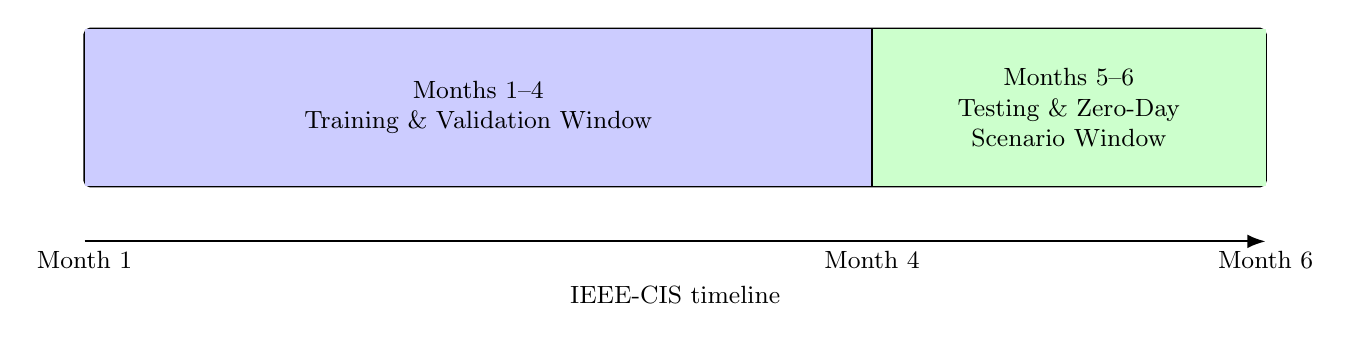
\begin{tikzpicture}[
  >=Latex,
  every node/.style={font=\small}
]
  \draw[thick, rounded corners=2pt] (0,0) rectangle (15,2.0);
  \fill[blue!20] (0,0) rectangle (10,2.0);
  \fill[green!20] (10,0) rectangle (15,2.0);
  \draw[thick] (10,0) -- (10,2.0);

  \node[align=center, text width=6.0cm] at (5,1.0) {Months 1--4\\Training \& Validation Window};
  \node[align=center, text width=4.4cm] at (12.5,1.0) {Months 5--6\\Testing \& Zero-Day\\Scenario Window};

  \draw[->, thick] (0,-0.7) -- (15,-0.7);
  \node[anchor=north] at (0,-0.7) {Month 1};
  \node[anchor=north] at (10,-0.7) {Month 4};
  \node[anchor=north] at (15,-0.7) {Month 6};
  \node[anchor=north] at (7.5,-1.15) {IEEE-CIS timeline};
\end{tikzpicture}
\caption{Chronological timeline for cross-temporal evaluation and zero-day testing.}
\label{fig:chronological-split}
\end{figure}

\section{Epoch-based Training Loop}
Weight persistence in Algorithm 1 is specifically included to capture slowly unfolding Account Takeover behavior. In practice, ATO attacks often begin with low-risk probing before transitioning to high-value abuse; carrying forward learned parameters across epochs helps the model accumulate these weak precursor signals instead of re-learning them from scratch in each snapshot.
\begin{algorithm}[h!]
\caption{Epoch-based training with graph rebuilding and weight persistence}
\begin{algorithmic}[1]
\State Initialize model parameters $\Theta$, DQN online network $\theta$, and target network $\theta^-$
\State Initialize experience replay buffer $\mathcal{D}$
\For{epoch $=1$ to $E$}
    \State Rebuild temporal graph snapshot from transactions in the current training window
    \State Keep learned model weights $\Theta$ and RL parameters $\theta$ from the previous epoch (weight persistence)
    \State Compute node embeddings using TSSGC with M-SEM fusion
    \State Infer dynamic channel weights and threshold actions via DQN policy
    \State Compute supervised fraud loss and RL reward
    \State Store transitions $(s_t,a_t,r_t,s_{t+1})$ in $\mathcal{D}$
    \State Sample mini-batch from $\mathcal{D}$ and minimize $\mathcal{L}_{\mathrm{DQN}}(\theta)$
    \State Update $\Theta$ using Adam optimizer and persist best checkpoint for progressively harder patterns (e.g., account takeover)
    \If{epoch mod $C = 0$}
        \State Update target network: $\theta^- \gets \theta$
    \EndIf
\EndFor
\end{algorithmic}
\end{algorithm}

\section{Planned Evaluation Methodology}
This section defines the planned evaluation protocol for measuring whether the proposed framework improves fraud detection quality under class imbalance and temporal drift. The goal is to evaluate practical robustness, not only point-in-time classification accuracy.

\subsection{Dataset Protocol}
Experiments are planned on the IEEE-CIS Fraud Detection dataset \cite{ieee_cis_dataset}, using \texttt{TransactionDT} to preserve time order. Following the cross-temporal setup in Section 4.3, data are split chronologically rather than randomly:
\begin{itemize}
    \item Training window: Months 1--4
    \item Validation split: Late portion of Months 1--4 (time-consistent tuning)
    \item Testing window: Months 5--6
\end{itemize}
Chronological splitting is essential because fraud distributions evolve over time. A random split can leak future patterns into training and overestimate real deployment performance under concept drift.

\subsection{Evaluation Metrics}
The planned metrics are AUC-ROC, AUC-PR, F1-score, and Recall@1\%.
\begin{itemize}
    \item \textbf{AUC-ROC}: overall ranking quality across thresholds.
    \item \textbf{AUC-PR}: emphasized because fraud data are highly imbalanced; precision-recall behavior is more informative for minority-class detection \cite{saito_pr_imbalanced}.
    \item \textbf{F1-score}: balance between precision and recall at an operating threshold.
    \item \textbf{Recall@1\%}: operational metric measuring how many fraud cases are captured when only the top 1\% highest-risk transactions can be investigated.
\end{itemize}

\subsection{Planned Baselines}
The proposed model will be compared against representative baselines from different methodological families:
\begin{itemize}
    \item Random Forest (tree-ensemble tabular baseline)
    \item XGBoost (strong tabular gradient-boosting baseline)
    \item GAT-based graph baseline (spatial graph learning without full proposed extensions)
    \item Original FraudGNN-RL framework (closest reference architecture)
\end{itemize}
These comparisons are intended to isolate gains from multi-modal semantic fusion and adaptive decision control.

\subsection{Robustness Evaluation Strategy}
Robustness will be evaluated through out-of-time testing and drift-aware scenarios:
\begin{itemize}
    \item \textbf{Out-of-time testing}: train on earlier months, test on later months.
    \item \textbf{Zero-day simulation}: treat newly emerging fraud patterns in Months 5--6 as unseen tactics at training time (consistent with Section~\ref{sec:fraud-taxonomy}).
    \item \textbf{Chronological generalization}: measure performance stability as temporal distance from training data increases.
\end{itemize}

\subsection{Computational Considerations}
Experiments are planned with GPU-accelerated mini-batch training. Practical constraints include graph memory footprint, epoch-wise graph rebuilding cost for temporal snapshots, and runtime trade-offs between model capacity and training stability.

\chapter{Conclusion \& Schedule}
\chapterdesc{This chapter summarizes the key contributions of the report and provides the implementation timeline for the next phase. It serves as the closing overview of what has been achieved and what will be completed in the planned roadmap.}

\section{Conclusion}
This report proposes a practical extension of FraudGNN-RL through multi-modal semantic fusion and adaptive control. By moving from shallow categorical entity embeddings to cross-modal behavioral-device semantic encoding, the framework is designed to improve sensitivity to identity camouflage while maintaining temporal robustness under concept drift.

The core contribution is the joint optimization synergy between representation learning and policy learning. The GNN branch learns \emph{what} is structurally and semantically suspicious by building high-quality node representations from temporal, spatial, and cross-modal signals. The RL branch learns \emph{how} to act on those representations under changing operating conditions, dynamically selecting thresholds and channel emphasis to balance fraud recall and false-positive cost. This two-level learning interaction yields a system that is more adaptive than static supervised pipelines and more interpretable than pure black-box threshold heuristics.

\section{Implementation Schedule}
\begin{table}[h!]
\centering
\caption{Implementation Schedule (4 Months)}
\begin{tabular}{@{}p{2cm}p{11cm}@{}}
\toprule
\textbf{Month} & \textbf{Activities} \\
\midrule
1 & Literature review and technical design finalization. \\
2 & IEEE-CIS preprocessing and feature engineering for semantic channels. \\
3 & Model integration: TSSGC + M-SEM + DQN-driven weighting. \\
4 & Evaluation, analysis, and report finalization. \\
\bottomrule
\end{tabular}
\end{table}

\clearpage
\phantomsection
\addcontentsline{toc}{chapter}{References}
\begin{thebibliography}{99}

\bibitem{rule_based_fraud}
Phua, C., Lee, V., Smith, K., and Gayler, R.:
\newblock A Comprehensive Survey of Data Mining-based Fraud Detection Research.
\newblock \emph{arXiv preprint arXiv:1009.6119}, 2010.

\bibitem{global_fraud_loss_report}
The Nilson Report:
\newblock Card Fraud Losses Worldwide --- 2024.
\newblock \emph{Nilson Report}, Issue 1298, December 2025.
\newblock URL: \url{https://nilsonreport.com/articles/card-fraud-losses-worldwide-2024/}.

\bibitem{saito_pr_imbalanced}
Saito, T. and Rehmsmeier, M.:
\newblock The Precision-Recall Plot Is More Informative than the ROC Plot When Evaluating Binary Classifiers on Imbalanced Datasets.
\newblock \emph{PLOS ONE}, 10(3):e0118432, 2015.

\bibitem{logistic_fraud}
Bhattacharyya, S., Jha, S., Tharakunnel, K., and Westland, J. C.:
\newblock Data mining for credit card fraud: A comparative study.
\newblock \emph{Decision Support Systems}, 50(3):602--613, 2011.

\bibitem{datamining_fraud}
Bolton, R. J. and Hand, D. J.:
\newblock Statistical fraud detection: A review.
\newblock \emph{Statistical Science}, 17(3):235--255, 2002.

\bibitem{ieee_cis_dataset}
Vesta Corporation and IEEE Computational Intelligence Society:
\newblock IEEE-CIS Fraud Detection Dataset.
\newblock Kaggle Competition Dataset, 2019.

\bibitem{rnn_fraud}
Jurgovsky, J., Granitzer, M., Ziegler, K., et al.:
\newblock Sequence Classification for Credit-Card Fraud Detection.
\newblock \emph{Expert Systems with Applications}, 100:234--245, 2018.

\bibitem{lstm_fraud}
Roy, A., Sun, J., Mahoney, R., et al.:
\newblock Deep learning detecting fraud in credit card transactions.
\newblock In \emph{Systems and Information Engineering Design Symposium (SIEDS)}, 2018.

\bibitem{adaboost_lstm}
Zhou, Y., Wang, H., and Li, X.:
\newblock AdaBoost-LSTM hybrid architecture for financial fraud detection.
\newblock \emph{Journal of Finance and Data Science}, 2021.

\bibitem{t_lstm}
Baytas, I. M., Xiao, C., Zhang, X., et al.:
\newblock Patient Subtyping via Time-Aware LSTM Networks.
\newblock In \emph{KDD}, 2017.

\bibitem{haint_lstm}
Zhang, Q., Liu, Y., and Chen, Z.:
\newblock HAInt-LSTM: Time-aware LSTM for irregular transaction behavior modeling.
\newblock \emph{IEEE Access}, 2022.

\bibitem{gnn_fraud_hetero}
Dou, Y., Liu, Z., Sun, L., et al.:
\newblock Enhancing Graph Neural Network-based Fraud Detectors against Camouflaged Fraudsters.
\newblock In \emph{CIKM}, 2020.

\bibitem{stgn}
Zhang, X., Xu, C., and Chawla, N. V.:
\newblock Spatial-Temporal Graph Neural Networks for Fraud Detection.
\newblock \emph{Proceedings of the AAAI Conference on Artificial Intelligence}, 2021.

\bibitem{tbhgn}
Li, J., Wang, S., and Liu, H.:
\newblock TbHGN: Temporal behavior hierarchical graph network for fraud detection.
\newblock \emph{Knowledge-Based Systems}, 2023.

\bibitem{th_gcl}
Wang, Y., Zhao, H., and Chen, L.:
\newblock TH-GCL: Temporal-Heterogeneous Graph Contrastive Learning for fraud detection.
\newblock \emph{Information Sciences}, 2024.

\bibitem{dqn}
Mnih, V., Kavukcuoglu, K., Silver, D., et al.:
\newblock Human-level control through deep reinforcement learning.
\newblock \emph{Nature}, 518(7540):529--533, 2015.

\bibitem{fraudgnn_rl}
Nguyen, T., Tran, P., and Le, H.:
\newblock FraudGNN-RL: Adaptive fraud detection with graph neural networks and deep reinforcement learning.
\newblock \emph{Expert Systems with Applications}, 2024.

\bibitem{fraudsentinel}
Patel, R., Kim, J., and Park, S.:
\newblock FraudSentinel: Federated multi-agent intelligence for cross-market fraud detection.
\newblock In \emph{IEEE International Conference on Big Data}, 2024.

\bibitem{fedavg}
McMahan, H. B., Moore, E., Ramage, D., Hampson, S., and y Arcas, B. A.:
\newblock Communication-efficient learning of deep networks from decentralized data.
\newblock In \emph{AISTATS}, 2017.

\end{thebibliography}

\end{document}
